\lab{Conditioning and Stability}{Conditioning and Stability}
\objective{Explore the condition of problems and the stability of algorithms.}
\label{lab:conditioning_stability}


%\begin{equation*}
%\mathlarger{ \mathlarger{ \mathlarger{f:X \rightarrow Y}}}
%\end{equation*}
%\begin{center} vs. \end{center}
%\begin{equation*}
%\mathlarger{ \mathlarger{ \mathlarger{\hat{f}:\hat{X} \rightarrow \hat{Y}}}}
%\end{equation*}

%\begin{eqnarray}
%\mathlarger{\mathlarger{\mathlarger{f:X \rightarrow Y}}}\\ \mathlarger{\mathlarger{\mathlarger{ f:\hat{X} \rightarrow \hat{Y} }}}\\
%\mathlarger{\mathlarger{\mathlarger{ \hat{f}:X \rightarrow Y }}}%\\
%%\mathlarger{\mathlarger{\mathlarger{ \hat{f}:\hat{X} \rightarrow \hat{Y} }}}
% \end{eqnarray}
% 

The \emph{condition number} of a function measures how sensitive that function is to changes in the input.
On the other hand, the \emph{stability} of an algorithm measures how well that algorithm computes the value of a function from exact input.

\section*{Condition Number of a Function}

The (absolute) condition number of a function $f: \mathbb{R}^m \rightarrow \mathbb{R}^n$ is
 \begin{equation}\label{equ:abs_cond}
J(\x) = \lim_{\delta \rightarrow 0} \sup_{\norm{\delta \x} \leq \delta} { \frac{\norm{\delta f}}{\norm{\delta \x}} } 
\end{equation}
where $\delta f = f(\x+\delta\x)-f(\x)$.
In other words, the condition number of $f$ is (the limit of) the change in output over the change of input.

Similarly, the \emph{relative condition number} of $f$ is the limit of the relative change in output over the relative change in input, i.e.,
\begin{equation}\label{equ:rel_cond}
\kappa(\x) = \lim_{\delta \rightarrow 0} \sup_{\norm{\delta \x} \leq \delta} \left({ \frac{\norm{\delta f}}{\norm{f(\x)}} } \middle/ { \frac{\norm{\delta \x}}{\norm{\x}} }\right).
\end{equation}
In fact,
\[
\kappa(\x) = \frac{\norm{\x}}{\norm{f(\x)}} J(\x)
\]
A function is \emph{ill-conditioned} if its condition number is large.


Small changes to the input of an ill-conditioned function produce large changes in output.
In applications, it is important to know if a function is ill-conditioned because there is usually some error in the parameters passed to the function.

\subsection*{Example: the Wilkinson Polynomial}

Let $f:\mathbb{C}^{n+1} \rightarrow \mathbb{C}^n$ be the function that sends $(a_1, \ldots, a_{m+1})$ to the roots of $a_1x^n+a_2x^{n-1}+\ldots+a_nx+a_{n+1}$.
In other words, this function describes the problem of finding the roots of a polynomial.
Unfortunately, root finding is extremely ill-conditioned.

A classic example is the Wilkinson polynomial 
\[
w(x) = \prod_{r=1}^{20}(x-r) = x^{20}-210x^{19}+20615x^{18}-\ldots.
\]
We will use NumPy to explore the condition number of $f$ at the coefficients of $w(x)$.
These coefficients are contained in the NumPy array \li{w_coeffs} below.
We also create an array \li{w_roots} containing the roots of $w(x)$.\footnote{
It is possible to create this array in NumPy by expanding the product $\prod_{r=1}^{20}(x-r)$, for example using \li{np.poly()}.
However, this approach is \emph{unstable} and will give you the wrong coefficients!}
\begin{lstlisting}
>>> import numpy as np
>>> from scipy import linalg as la
>>> w_coeffs = np.array([1, -210, 20615, -1256850, 53327946, -1672280820,
                    40171771630, -756111184500, 11310276995381,
                    -135585182899530, 1307535010540395,
                    -10142299865511450, 63030812099294896,
                    -311333643161390640, 1206647803780373360,
                    -3599979517947607200, 8037811822645051776,
                    -12870931245150988800, 13803759753640704000,
                    -8752948036761600000, 2432902008176640000])
>>> w_roots = np.arange(1, 21)
\end{lstlisting}

Next we perturb the polynomial by changing the $x^{19}$-coefficient from $-210$ to $-210.0000001$.
\begin{lstlisting}
>>> perturb = np.zeros(21)
>>> perturb[1]=1e-7
>>> perturbed_coeffs = w_coeffs - perturb
\end{lstlisting}

Now we find the roots of the perturbed polynomial.
The function \li{np.poly1d()} creates a polynomial object using the array passed to it as coefficients, and \li{np.roots()} finds the roots of a polynomial.
\begin{lstlisting}
>>> perturbed_roots = np.roots(np.poly1d(perturbed_coeffs))
\end{lstlisting}
The new roots are plotted with the original roots in Figure \ref{fig:wilkinsonpolynomial}.

Finally we compute an approximation to the condition number.
We sort the roots before we compare them to ensure that they are in the same order.
\begin{lstlisting}
>>> w_roots = np.sort(w_roots)
>>> perturbed_roots = np.sort(perturbed_roots)
>>> la.norm(perturbed_roots-w_roots)/la.norm(perturb)
68214100.15878984
\end{lstlisting}
Thus, the condition number of this problem is something like $10^7$. 

When we try to estimate the relative condition number, NumPy will not compute the 2-norm of \li{w_coeffs} because it is so large.
NumPy will not compute the square root of a very large number.
One easy solution is to use a different norm that does not require the square root. 
\begin{lstlisting}
>>> # Estimate the absolute condition number in the infinity norm
>>> k = la.norm(perturbed_roots-w_roots, np.inf)/la.norm(perturb, np.inf)
>>> k
28260604.34345689
>>> # Estimate the relative condition number in the infinity norm
>>> k*la.norm(w_coeffs, np.inf)/la.norm(w_roots, np.inf)
1.9505129642488696e+25
\end{lstlisting}
As you can see, the order of magnitude of the absolute condition number is the same as when we computed it with the 2-norm.
The relative condition number for this problem is approximately $10^{24}$.


There are some caveats to this example. 
First, when we compute the quotients in \eqref{equ:abs_cond} and \eqref{equ:rel_cond} for a fixed $\delta \x$, we are only \emph{approximating} the condition number.
The actual condition number is a limit of such quotients.
We hope that when $||\delta \x||$ is small, a random quotient is at least the same order of magnitude as the limit, but we have no way to be sure.

Second, this example assumes that NumPy's root-finding algorithm is \emph{stable}, so that the difference between the roots of \li{w_coeffs} and \li{perturbed_coeffs} is due to the difference in coefficients, and not the difference in roots.
We will return to this issue in the next section.

\begin{figure}
\centering
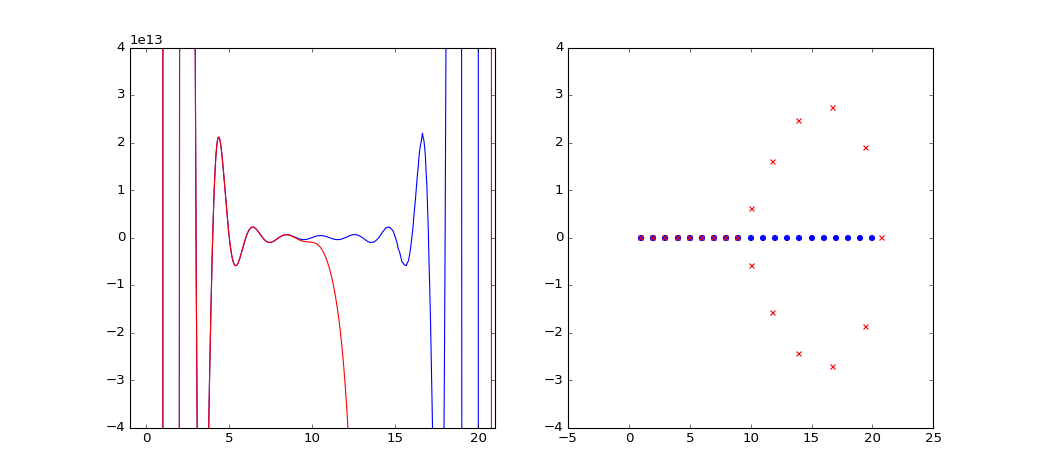
\includegraphics[height=2.25in]{wilk2.png}
\caption{In these images, blue is associated with $w(x)$ and red is associated with $w(x)$ perturbed by 1e-7 in the $x^{19}$-coefficient. On the left is a plot of the two polynomials. On the right is a graphical representation of the roots of the polynomials. The blue dots are the roots of $w(x)$. The red x's are the roots of the perturbed polynomial. }
\label{fig:wilkinsonpolynomial}
\end{figure}

\begin{problem}\label{prob:wilk}
Write a Python function that investigates the condition number of the Wilkinson polynomial by doing the following.
\begin{enumerate}
\item Perform this experiment:

\begin{quote}
Randomly perturb $w(x)$ by replacing each coefficient $a_i$ with $a_i*r_i$, where $r_i$ is drawn from a normal distribution centered at 1 with standard deviation $1e-10$.
\end{quote}

Plot the results of 100 such experiments in a single graphic, along with the roots of the unperturbed polynomial $w(x)$. The plot should look something like Figure \ref{fig:wilkinsonpolynomial_many}. This exercise reproduces Figure 12.1 on p. 93 of \emph{Numerical Linear Algebra} by Lloyd N. Trefethen and David Bau III.
\item Using the final experiment only, estimate the relative and absolute condition number (in any norm you prefer). Print these numbers to the screen.
\end{enumerate}
\begin{figure}[H]
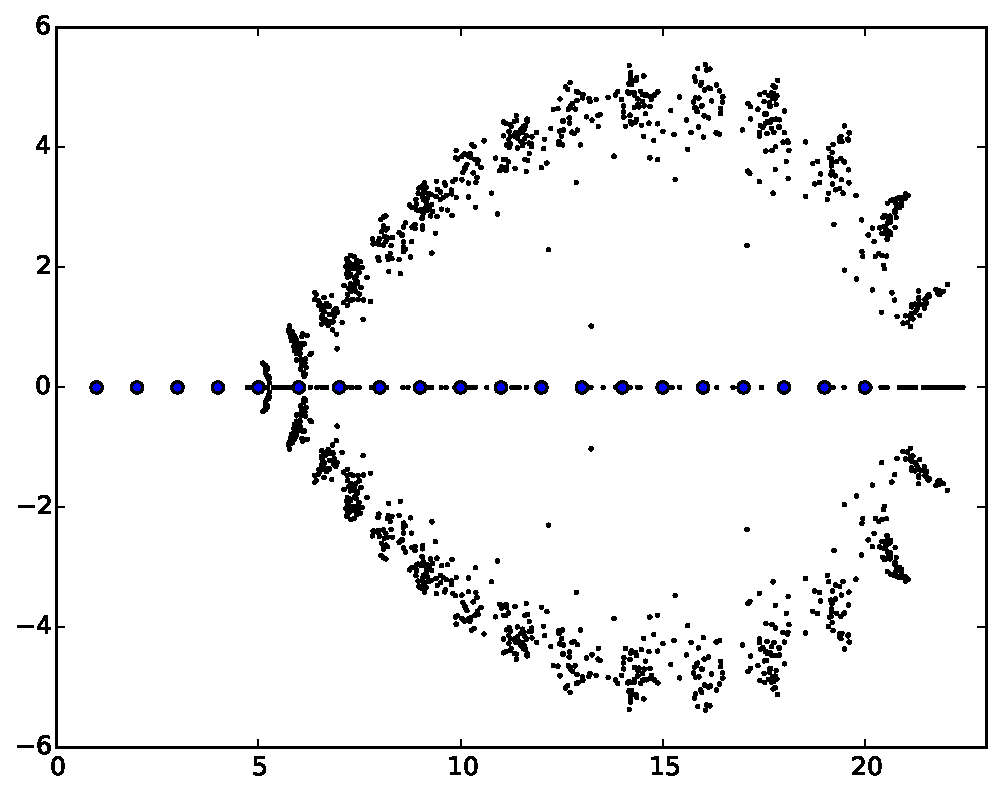
\includegraphics[height=3in]{wilkinsonpolynomial_many.pdf}
\caption{Sample result of Problem \ref{prob:wilk}.
The blue dots are the roots of $w(x)$ and the black dots are roots of random perturbations. 
This figure replicates Figure 12.1 on p. 93 of \emph{Numerical Linear Algebra} by Lloyd N. Trefethen and David Bau III.}
\label{fig:wilkinsonpolynomial_many}
\end{figure}

\end{problem}

%Notes on Problem 1:
% - Make something to copy-paste with the polynomial coefficients
% - You MUST copy paste the exact coefficients!!! Multiplying out the polynomial is not stable!!!
% - Also "compute" the roots of the wilkinson poly. They are close but not quite right. The difference is not visible on the graph. See that is probably useful.

% In introductory discussion, compute the condition number of the problem. Explain why we use the infinity norm.

\subsection*{Example: Calculating Eigenvalues}

Let $f:\mathbb{C}^{n^2} \rightarrow \mathbb{C}^n$ be the function that sends an $n \times n$ matrix to its $n$ eigenvalues.
This problem is well-conditioned for symmetric matrices, but can be extremely ill-conditioned for non-symmetric matrices.

Let us use NumPy to calculate the condition number of the eigenvalue problem at the identity matrix.
First we check that the eigenvalue solver is stable here.
\begin{lstlisting}
>>> M = np.array([[1,0],[0,1]])
>>> eigs = la.eig(M)[0]
>>> eigs
array([ 1.+0.j,  1.+0.j])
\end{lstlisting}
Now we perturb $M$ by adding a matrix drawn from a random normal distribution over the complex numbers.
We calculate the eigenvalues of the perturbed matrix.
\begin{lstlisting}
>>> perturb = np.random.normal(0, 1e-10, M.shape) + np.random.normal(0,1e-10, M.shape)*1j
>>> eigsp = la.eig(M+perturb)[0]
\end{lstlisting}
Finally we use this data to approximate the condition number.
\begin{lstlisting}
>>> k = la.norm(eigs-eigsp)/la.norm(perturb)	# Absolute condition number
0.62957336119253127
>>> k*la.norm(M)/la.norm(eigs)	# Relative condition number
0.62957336119253127
\end{lstlisting}
The absolute and relative condition number are the same because \li{la.norm(M)} and \li{la.norm(eigs)} are both $\sqrt{2}$.


\begin{problem}[Optional]\label{prob:eigenvalue}
Let us explore the condition number of the eigenvalue problem.
\begin{enumerate}
\item \begin{enumerate}
\item Write the following function.
\begin{lstlisting}
def eig_condit(M):
    '''
    Approximate the condition number of the eigenvalue problem at M.
    
    INPUT:
    M  - A 2-D NumPy array, representing a matrix.
    
    RETURN:
    A tuple containing approximations to the absolute and relative condition numbers of the eigenvalue problem at M.
    '''
\end{lstlisting}
\item Find an example of a $2\times2$ matrix with a very large condition number. 
(Hint: Look at matrices whose off-diagonal entries are very different in magnitude.)
\item What is the order of magnitude of the condition number of a symmetric $2\times 2$ matrix?
\end{enumerate}
\item Write the following function.
\begin{lstlisting}
def plot_eig_condit(x0=-100, x1=100, y0=-100, y1=100, res=10):
    '''
    Plot the condition number of the eigenvalue problem on [x0, x1]x[y0,y1].
    
    Specifically, use plt.pcolormesh to plot the relative condition number of the eigenvalue problem at [[1,x],[y,1]] on this domain.
    The variable `res' should be the number of sample points taken along each axis, for a total of `res'**2 points in the plot.
    '''
\end{lstlisting}
\item Call your function for \li{res}=10, 50, 100, 200 and 400 (output for $res=200$ is pictured below). Recall that matplotlib scales the colorbar of the output to fit the largest and smallest output values.
What can you conclude about the condition number of the eigenvalue problem at a ``random'' $2\times2$ matrix?
\end{enumerate}
\begin{figure}[H]
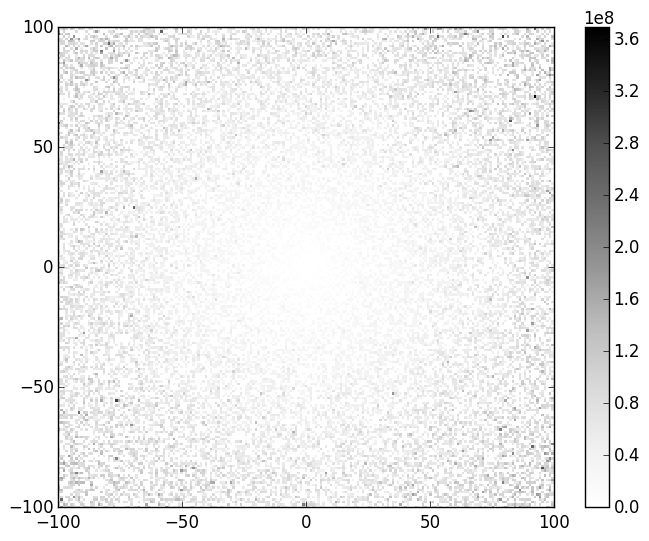
\includegraphics[height=3in]{eigenvalue_conditioning.png}
\caption{Output of \li{plot_eig_condit(res=200)}.}
\end{figure}
\end{problem}

%\begin{example}[Condition of a System of Equations]
%Consider the system of equations
%\[ Ax = b \] 
%for an $n \times n$ matrix $A$ and $n \times 1$ vectors $x$ and $b$. If we hold $A$ fixed, consider the problem of computing $b$ with respect to small changes in $x$. Alternatively, hold $A$ fixed and consider the problem of computing $x = A^{-1} b$ with respect to small changes in $b$. Finally, we may hold $b$ fixed and consider the problem of computing $x = A^{-1}b$ with respect to small changes in $A$.
%
%It turns out that each of these problems has the \emph{same} relative condition number. This number is 
%\[
%\mathcal{K} (A) = \norm{A}_2 \norm{A^{-1}}_2
%\]
%
%This is called the \emph{condition number of $A$}.
%The condition number of a matrix can be computed using \li{numpy.linalg.cond()}.
%
%Notice that the condition number of a matrix cannot be less that $1$.
%It is almost always best to work with orthonormal matrices (or operations that can be mathematically represented by orthonormal matrices).
%Since orthonormal matrices have a norm of $1$, as do their inverses, these transformations have the best possible condition number.
%The low condition number of orthonormal matrices is one of the primary reasons that Householder reflections and Givens rotations are used in so many algorithms.
%\end{example}

\section*{Stability of an Algorithm}

The stability of an algorithm is measured by the error in its output. 
Suppose we have some algorithm to compute $f: \mathbb{R}^m \rightarrow \mathbb{R}^n$.
Let $\tilde f(\x)$ represent the value computed by the algorithm at $\x$.
Then the \emph{forward error} of $f$ at $\x$ is $||f(\x)-\tilde f(\x)||$, and the \emph{relative forward error} of $f$ at $\x$ is
\[
\frac{||f(\x)-\tilde f(\x)||}{||f(\x)||}.
\]
An algorithm is \emph{stable} if this relative forward error is small.

As an example, let us examine the stability of NumPy's root finding algorithm that we used to investigate the Wilkinson polynomial.
We know the exact roots of $w(x)$, and we can also compute these roots using NumPy's \li{np.roots()} function.

\begin{lstlisting}
>>> roots = np.arange(1,21)
>>> w_coeffs = np.array([1, -210, 20615, -1256850, 53327946, -1672280820,
                    40171771630, -756111184500, 11310276995381,
                    -135585182899530, 1307535010540395,
                    -10142299865511450, 63030812099294896,
                    -311333643161390640, 1206647803780373360,
                    -3599979517947607200, 8037811822645051776,
                    -12870931245150988800, 13803759753640704000,
                    -8752948036761600000, 2432902008176640000])
>>> computed_roots = np.roots(np.poly1d(w_coeffs))
\end{lstlisting}

We sort the roots to ensure they are in the same order, then compute the absolute and relative forward error.

\begin{lstlisting}
>>> roots = np.sort(roots)
>>> computed_roots = np.sort(computed_roots)
>>> la.norm(roots-computed_roots)	# Forward error
0.020612653126379665
>>> la.norm(roots-computed_roots)/la.norm(roots)	# Relative forward error
0.00038476268486104599
\end{lstlisting}

This analysis gives us hope that questions of stability did not interfere too much with our experiments in Problem \ref{prob:wilk}.

\subsection*{Catastrophic Cancellation}
\emph{Catastrophic Cancellation} is a term for when a computer takes the difference of two very similar numbers, and the result is stored with a small number of significant digits.
Because of the way computers store and perform arithmetic on numbers, future computations can amplify a catastrophic cancellation into a huge error.

You are at risk for catastrophic cancellation whenever you subtract floats or large integers that are very close to each other.
You can avoid the problem either by rewriting your program to not use subtraction, or by increasing the number of significant digits that your computer tracks.

Here is an example of catastrophic cancellation.
Suppose we wish to compute $\sqrt{a}-\sqrt{b}$. We can either do this subtraction directly or perform the equivalent division
\[
\sqrt{a}-\sqrt{b} = (\sqrt{a}-\sqrt{b})\frac{\sqrt{a}+\sqrt{b}}{\sqrt{a}+\sqrt{b}} = \frac{a-b}{\sqrt{a}+\sqrt{b}}.
\]

Let us perform this computation both ways in NumPy with $a=10^{20}+1$ and $b=10^{20}$.
\begin{lstlisting}
>>> np.sqrt(1e20+1)-np.sqrt(1e20)
0.0
>>> 1/(np.sqrt(1e20+1)+np.sqrt(1e20))
5.0000000000000002e-11
\end{lstlisting}
Since $a \neq b$, clearly $\sqrt{a}-\sqrt{b}$ should be nonzero. 


\begin{problem}
Let $I(n) = \int_0^1 x^n e^{x - 1} dx$.
\begin{enumerate}
\item Prove that $0 \leq I(n) \leq 1$ for all $n$.
\item It can be shown that for $n>1$, 
\[
I(n) = \left(-1\right)^{n} !n + \left(-1\right)^{n + 1} \frac{n!}{e}
\]
where $!n$ is the \emph{subfactorial} of $n$. 
Use this formula to write the following function.
\begin{lstlisting}
def integral(n):
    '''Return I(n).'''
\end{lstlisting}
Hint: The subfactorial function can be imported from SymPy with the line \li{from sympy import subfactorial}.
\item The actual values of $I(n)$ for many values of $n$ are listed in the table below.
Use your function \li{integral()} to compute $I(n)$ for these same values of $n$, and create a table comparing the data.
How can you explain what is happening?
\end{enumerate}

\begin{center}
\begin{tabular}{|l|l|}
\hline
$n$  & Actual value of $I(n)$ \\
\hline
$1$  & $0.367879441171$ \\
$5$  & $0.145532940573$ \\
$10$ & $0.0838770701034$ \\
$15$ & $0.0590175408793$ \\
$20$ & $0.0455448840758$ \\
$25$ & $0.0370862144237$ \\
$30$ & $0.0312796739322$ \\
$35$ & $0.0270462894091$ \\
$40$& $0.023822728669$ \\
$45$& $0.0212860390856$ \\
$50$ & $0.0192377544343$ \\
\hline
\end{tabular}
\end{center}

\end{problem}

%\begin{table}
%\centering
%\begin{tabular}{|l|l|l|}
%\hline
%Integrand & Computed Value & Actual Value \\
%\hline
%$x^{1}e^{x}$: & $0.367879441171$ & $0.367879441171$ \\
%$x^{5}e^{x}$: & $0.145532940573$ & $0.145532940573$ \\
%$x^{10}e^{x}$: & $0.0838770701084$ & $0.0838770701034$ \\
%$x^{15}e^{x}$: & $0.0590209960938$ & $0.0590175408793$ \\
%$x^{20}e^{x}$: & $0.0$ & $0.0455448840758$ \\
%$x^{25}e^{x}$: & $1073741824.0$ & $0.0370862144237$ \\
%$x^{30}e^{x}$: & $-1.80143985095 \cdot 10^{16}$ & $0.0312796739322$ \\
%$x^{35}e^{x}$: & $6.04462909807 \cdot 10^{23}$ & $0.0270462894091$ \\
%$x^{40}e^{x}$: & $0.0$ & $0.023822728669$ \\
%$x^{45}e^{x}$: & $0.0$ & $0.0212860390856$ \\
%$x^{50}e^{x}$: & $1.46150163733 \cdot 10^{48}$ & $0.0192377544343$ \\
%\hline
%\end{tabular}
%\caption{Inaccuracy of values computed using an unstable algorithm.}
%\label{table:unstable_computation}
%\end{table}

% For this section to be meaningful, it needs more explanation of when each algorithm is stable.
\begin{comment}
The algorithms that we have studied to solve linear systems have different levels of stability.
LU decomposition (with pivoting) is usually good enough, but there are some pathological examples of matrices that cause it to break down.
QR decomposition (with pivoting) is generally considered to be a better option than the LU decomposition.
Solving a linear system using the SVD is even more stable than the QR decomposition.
(Pivoting is a modification that is commonly made to the LU decomposition and QR decomposition algorithms we have discussed in earlier labs to make them more stable.)
Unfortunately, in this case, the algorithms that are more stable are also slower.
The LU decomposition is used by \li{scipy.linalg.solve()}.
The SVD is used by \li{scipy.linalg.lstsq()}.
Here is some code that uses the QR decomposition of a matrix $A$ to solve the linear system $A x = b$ for $x$.
It uses a lower-level function included in SciPy to perform the back substitution required to solve this system.
\begin{lstlisting}
from scipy import linalg as la
from scipy.linalg.flapack import dtrtrs
def qr_solve(A, b):
    Q, R = la.qr(A)
    return dtrtrs(R.T, Q.T.dot(b), lower=1, trans=1)[0]
\end{lstlisting}
A solution using a pivoted QR decomposition would be better, but this will be good enough for demonstration purposes.

The following are routines that generate matrices designed to show the relative benefits of each of these algorithms.
\begin{lstlisting}
from numpy.random import rand

def bad_arr_1(n):
    """ Construct a specific pathological example
    that breaks LU decomposition. These examples
    are very rare, but they do exist.
    Strictly speaking, the condition number
    for this matrix isn't terribly bad. """
    A = - np.ones((n, n))
    A[:,:-1] = np.tril(A[:,:-1])
    np.fill_diagonal(A, 1)
    A[:,-1] = 1
    return A

def bad_arr_2(n, peturbation = 1E-8):
    """ Construct another matrix that is nearly singular
    by computing A.dot(A.T) for a matrix A that is
    not square and then adding some small changes
    so it is not exactly singular. """
    A = rand(n, n // 2)
    return A.dot(A.T) + peturbation * rand(n, n)
\end{lstlisting}
\end{example}

\begin{problem}
For each of the array creation routines above, plot the error $\norm{\text{solve}\left(A, A b\right) - b}$ of each of the methods mentioned above for solving a linear system.
Use a log-scaled $y$-axis.
What do you observe?
\end{problem}
\end{comment}
%\subsection*{Stable vs. Backward Stable Algorithms}

%\subsection*{Table}
%
%\begin{table}[h]
%\begin{tabular}{|l|l|l|}
%\hline \textbf{Well-Conditioned} & \textbf{Ill-Conditioned} & \textbf{Systems of Equations} \\
%{\parbox{0.3\textwidth}{\raggedleft
%            \begin{itemize}[leftmargin=*]
%                \item finding eigenvalues of a symmetric (or normal) matrix 
%                \item calculating $e^x$ for relatively small values of $x$ 
%                \item calculating $\ln(x)$ for $x$ not close to $1$
%            \end{itemize} }}           &  
%             
%{\parbox{0.3\textwidth}{\raggedleft
%            \begin{itemize}[leftmargin=*]
%                \item calculating $x_1 - x_2$ when $x_1 \approx x_2$ 
%                \item computing roots of a polynomial, given the coefficients
%                \item computing eigenvalues of a non-symmetric matrix
%            \end{itemize} }}              &   
%            
%{\parbox{0.3\textwidth}{
%            \begin{itemize}[leftmargin=*]
%                 \item relative condition number is \[ \mathcal{K} = ||A|| ||A^{-1}|| \]
%            \end{itemize} }}   \\ \hline                      
%\end{tabular}
%\end{table}
%
%
%\begin{table}[h]
%\begin{tabular}{|l|l|}
%\hline \textbf{Stable} & \textbf{Unstable} \\
%{\parbox{0.45\textwidth}{\raggedleft
%            \begin{itemize}[leftmargin=*]
%                \item finding eigenvalues of a symmetric (or normal) matrix 
%                \item calculating $e^x$ for relatively small values of $x$ 
%                \item calculating $\ln(x)$ for $x$ not close to $1$
%            \end{itemize} }}           &  
%             
%{\parbox{0.45\textwidth}{\raggedleft
%            \begin{itemize}[leftmargin=*]
%                \item calculating $x_1 - x_2$ when $x_1 \approx x_2$ 
%                \item computing roots of a polynomial, given the coefficients
%                \item computing eigenvalues of a non-symmetric matrix
%            \end{itemize} }}    \\ \hline                      
%\end{tabular}
%\end{table}
%
